\documentclass[a0,landscape]{a0poster}
\usepackage{times}
\usepackage{graphicx}
\usepackage{multicol}
\usepackage{geometry}
\usepackage{qrcode}
\usepackage{amssymb}
\usepackage[most]{tcolorbox}
\usepackage{alltt}

% --- Page Geometry (Set to 48x36 inches with a 1-inch margin) ---
\geometry{papersize={48in,36in}, margin=1in}

% --- Custom Box Style ---
\newtcolorbox{posterbox}[1]{
    colback      = blue!5!white,
    colframe     = blue!75!black,
    fonttitle    = \bfseries,
    title        = {#1},
    breakable,
    boxsep       = 8mm,
    arc          = 5mm,
}

\begin{document}

% === TITLE BLOCK ===
\begin{center}
    \veryHuge \textbf{RMSTSS: A New Tool for Planning Better, Faster Medical Studies} \\
    \vspace{0.25cm}
    \rule{\linewidth}{1.5pt}
    \vspace{0.25cm}
    \Huge \textbf{Arnab Aich} \\
     \textit{University of Tennessee Health Science Center}
\end{center}

\vspace{0.5cm}

% === 3-COLUMN LAYOUT ===
\begin{multicols}{3}

% --- COLUMN 1 ---
\begin{posterbox}{From Trial Setup to a Better Metric}

    \subsection*{ Basic Setup of a Clinical Trial}
    
    In many studies, we compare two groups of patients:
    \begin{itemize} \itemsep=0.5em
        \item A \textbf{Treatment} group receiving a new medicine.
        \item A \textbf{Control} group receiving a placebo or standard care.
    \end{itemize}
    We then follow them over time to measure a **time-to-event** endpoint, such as time to recovery or survival time.

    \vspace{0.5cm}\hrule\vspace{0.5cm}

    \subsection*{ The Core Challenge: Study Design}
    
    Before starting, researchers must answer two critical questions:
    \begin{enumerate} \itemsep=0.5em
        \item \textbf{Sample Size:} "How many patients do we need for a reliable result?"
        \item \textbf{Power:} "Given our patients, what is our chance of success?"
    \end{enumerate}
    Answering these questions correctly is essential for an ethical and cost-effective study.

    \vspace{0.5cm}\hrule\vspace{0.5cm}
    
     \subsection*{ Why Traditional Methods Can Be Problematic}
    
    For decades, clinical trials have relied on two main approaches:
    \begin{itemize} \itemsep=0.75em
        \item \textbf{Hazard Ratio (HR):} This popular metric relies on a strong statistical assumption (proportional hazards) that is often violated in the real world. When this happens, the HR loses its clear meaning.
        \item \textbf{Direct Survival Modeling:} Comparing survival at a single point (e.g., 5-year survival) ignores the patient's journey and can be misleading.
    \end{itemize}
    
    \vspace{0.5cm}\hrule\vspace{0.5cm}

    \subsection*{ A Better Metric: RMST}
    
    Instead of complex metrics, we can use **RMST** (Restricted Mean Survival Time). It directly measures the average "event-free" time patients experience. It is a good measure because it:
    \begin{itemize} \itemsep=0.5em
        \item[\checkmark]  Is easy for everyone to understand.
        \item[\checkmark]  Provides a clear measure of treatment benefit.
    \end{itemize}
    
    \begin{center}
        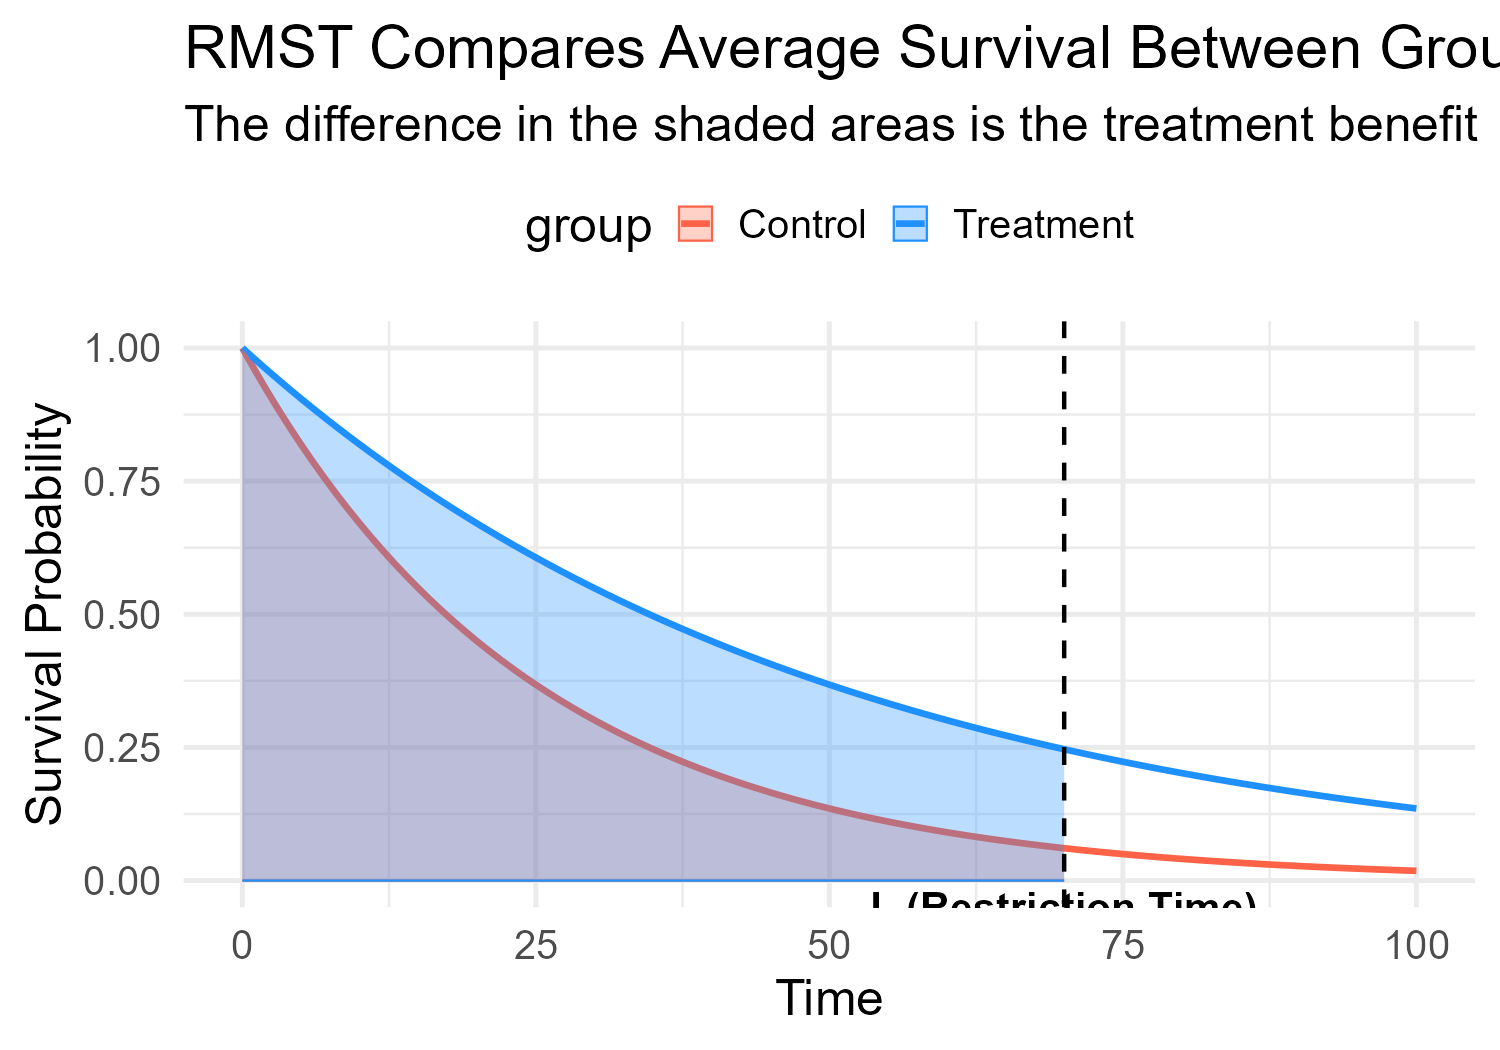
\includegraphics[width=0.9\linewidth]{rmst_causal_plot.png}
    \end{center}
\end{posterbox}



\columnbreak

% --- COLUMN 2 ---
\begin{posterbox}{Our Solution: The RMSTSS Tool}
    
    Planning studies with RMST has been difficult. We made it easy. `RMSTSS` is a free tool that helps researchers properly plan modern medical studies.
    
    \begin{center}
        \vspace{0.5cm}
        % Make sure you have an image named 'app-sc.png' in your folder
        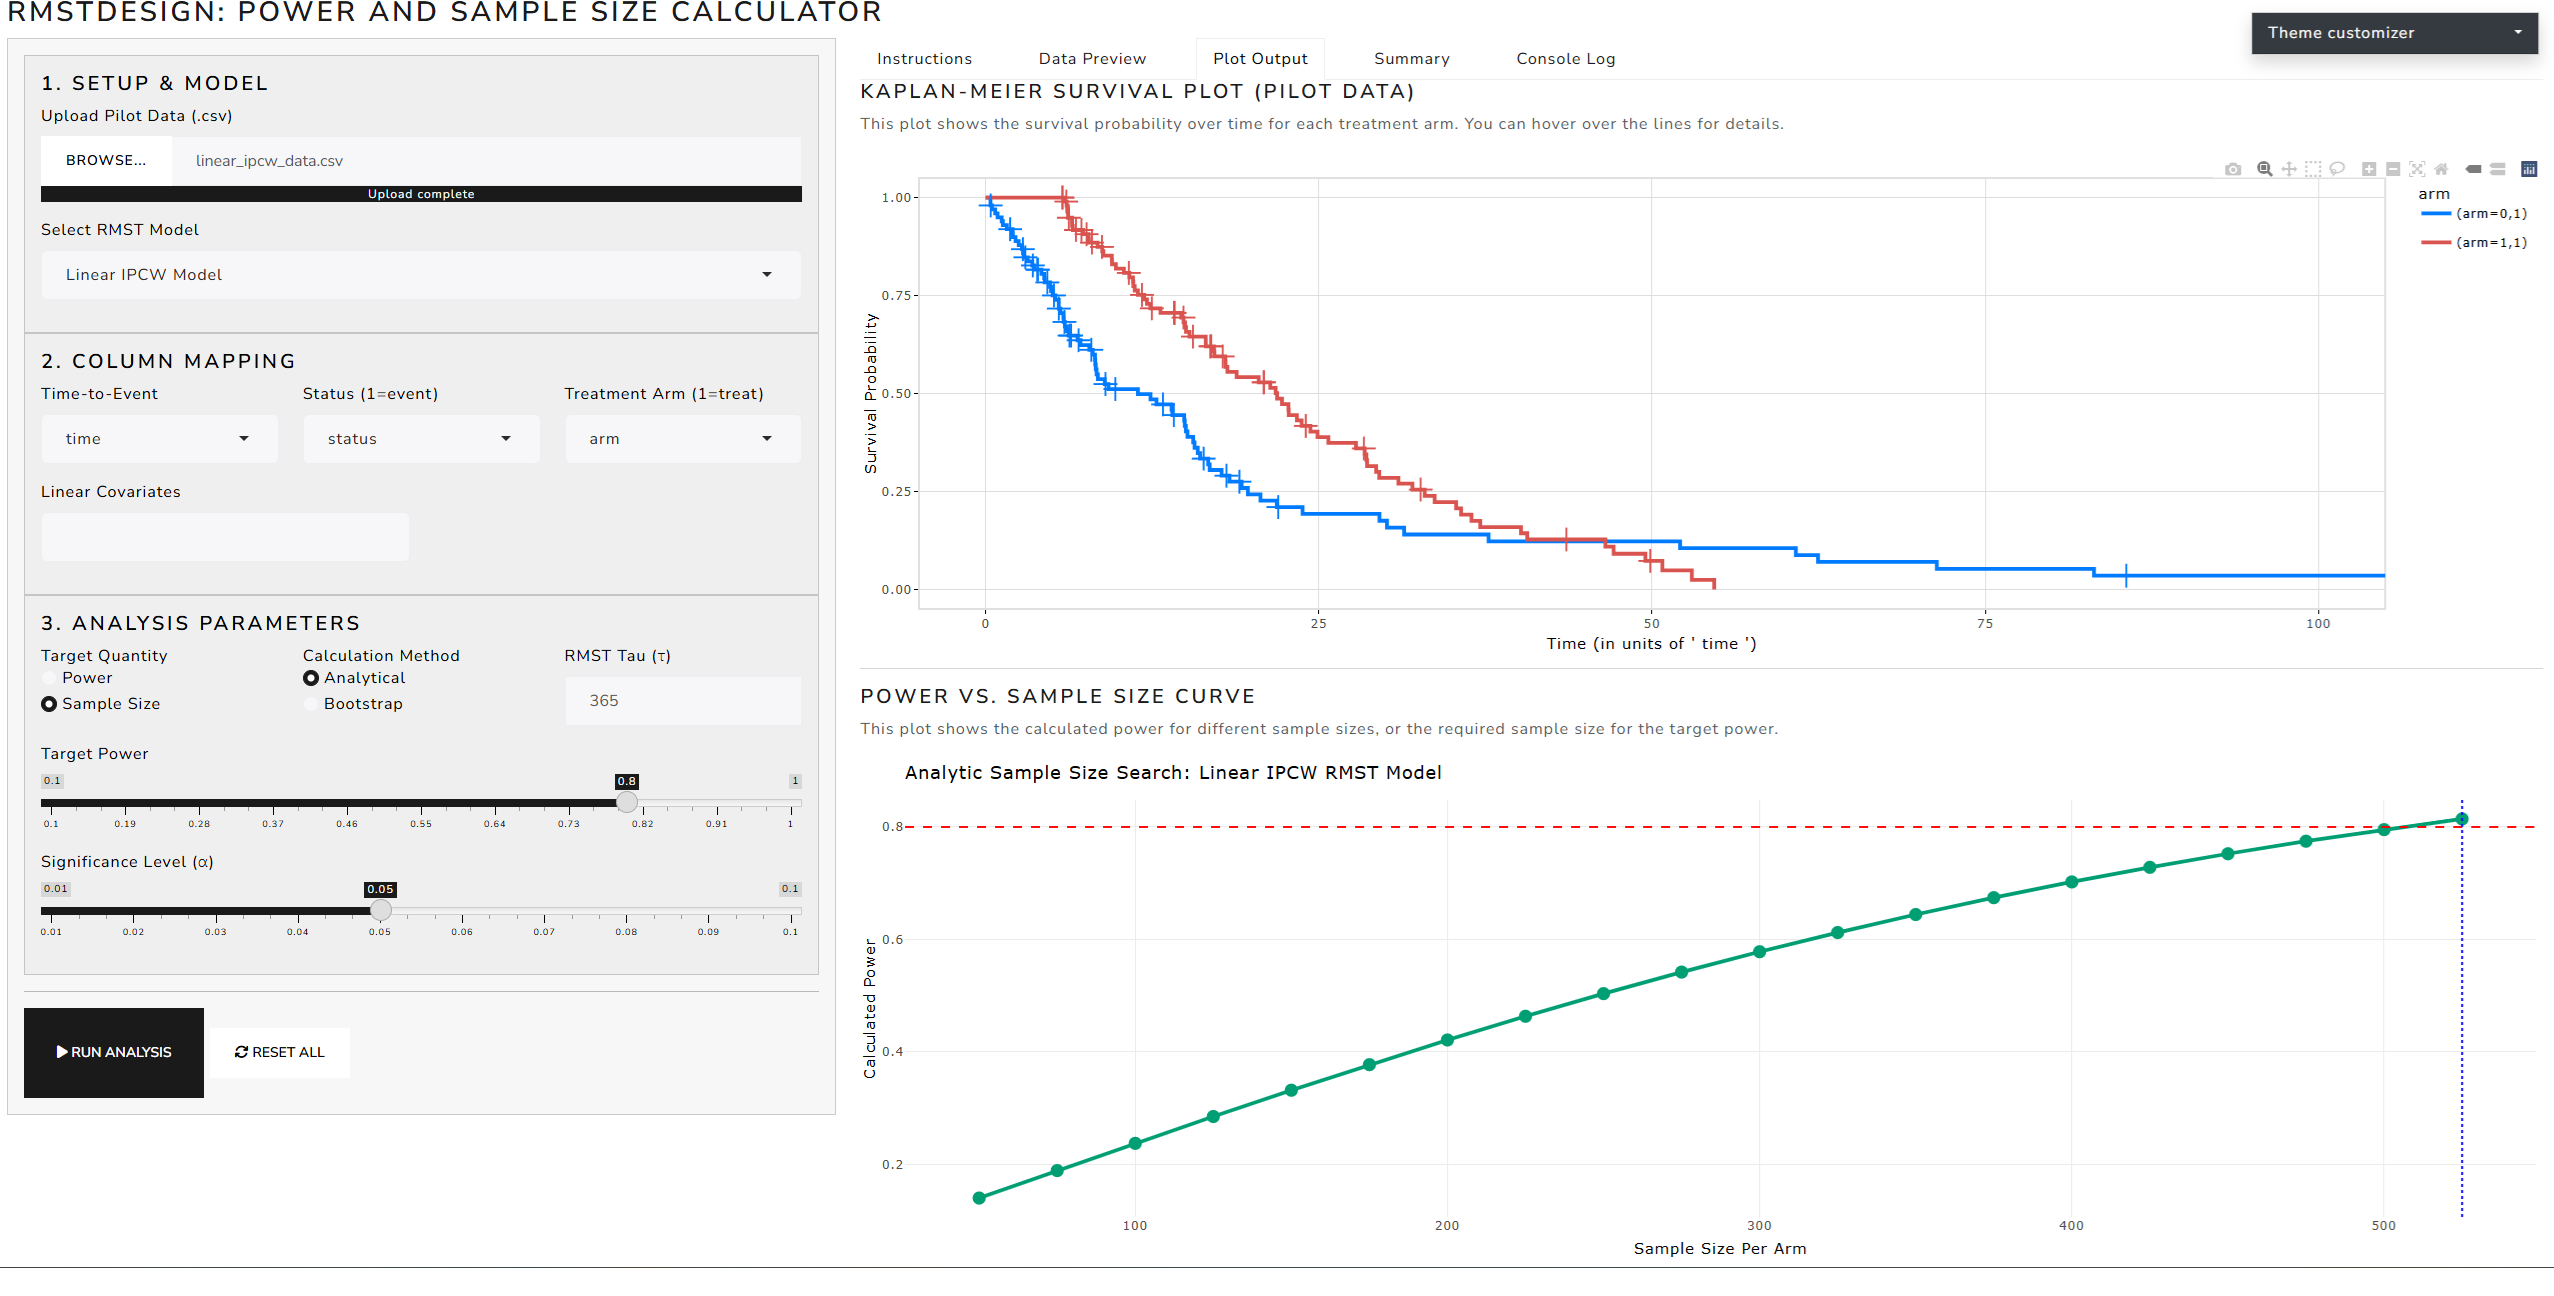
\includegraphics[width=0.9\linewidth]{app-ss.png}
        \vspace{0.5cm}
    \end{center}
    
    \subsection*{ How to Use the App}
    The web application guides you through the process in a left-to-right flow:
    \begin{center}
        
        \begin{tabular}{ccccccc}
            \textbf{Upload Data} &  $\boldsymbol{\rightarrow}$ & \textbf{Choose Model} &  $\boldsymbol{\rightarrow}$ & \textbf{Choose Target}  $\boldsymbol{\rightarrow}$ & \textbf{Get Results} \\
        \end{tabular}
    \end{center}
\end{posterbox}

\begin{posterbox}{Features \& Capabilities}
    \subsection*{ A Full Suite of Modern Models}
    
    Our tool handles many real-world research scenarios:
    \begin{itemize} \itemsep=0.75em
        \item \textbf{Linear Model}: For standard clinical trials.
        \item \textbf{Stratified Models}: For studies run at many different hospitals.
        \item \textbf{GAM Model}: For studies where factors like patient age have complex effects.
        \item \textbf{Dependent Censoring}: For studies with competing outcomes, like transplants.
    \end{itemize}

    \subsection*{ Choose Your Goal}
    
    \begin{itemize} \itemsep=0.75em
        \item \textbf{Power Calculation}: Find the chance of success for a given study size.
        \item \textbf{Sample Size Search}: Find how many patients you need to succeed.
    \end{itemize}

    \subsection*{ Choose Your Method}
    
    \begin{itemize} \itemsep=0.75em
        \item \textbf{Quick Check (Analytical)}: A fast answer for exploring ideas.
        \item \textbf{Deep Dive (Bootstrap)}: A powerful simulation for a more accurate result. Our tool can run these simulations in parallel to be faster!
    \end{itemize}
\end{posterbox}

\columnbreak


% --- COLUMN 3 ---
\begin{posterbox}{The RMSTSS R Package}
    \huge
    For statisticians and developers, `RMSTSS` is available as a powerful and flexible R package for use in scripts and analysis pipelines.
    
    \subsection*{\huge Key Functions \& When to Use Them}
    \Large
    The package provides a suite of functions for different trial designs:
    
    \vspace{0.5cm}
    \begin{tabular}{|p{5cm}|p{7cm}|}
        \hline
        \textbf{\large Function Group} \& \textbf{\large Use Case} \\
        \hline
        \texttt{linear.*()} \& Standard clinical trials with linear effects. \\ \hline
        \texttt{additive.*()} \& Multi-hospital trials with a constant treatment benefit. \\ \hline
        \texttt{MS.*()} \& Multi-hospital trials with a proportional treatment benefit. \\ \hline
        \texttt{GAM.*()} \& When factors like patient age may have complex, non-linear effects. \\ \hline
        \texttt{DC.*()} \& Studies with competing outcomes, such as organ transplants. \\
        \hline
    \end{tabular}

    \subsection*{\huge Installation Guide}
    \Large
    Install the development version directly from GitHub with this command:
    \begin{alltt}
remotes::install_github(
  "UTHSC-Zhang/RMSTSS-Package"
)
    \end{alltt}

    \subsection*{\huge Access Links}
    \begin{center}
    \begin{tabular}{cc}
        % GitHub QR Code
        \begin{minipage}{0.45\linewidth}
            \centering
            \qrcode[height=5cm]{https://github.com/UTHSC-Zhang/RMSTSS-Package}
        \end{minipage}
        &
        % Web App QR Code
        \begin{minipage}{0.45\linewidth}
            \centering
            \qrcode[height=5cm]{https://arnab96.shinyapps.io/uthsc-app/}
        \end{minipage}
        \\
    \end{tabular}
    \end{center}
\end{posterbox}

\end{multicols}
\end{document}
